\setlength{\parindent}{3ex}
\setlength{\parskip}{0ex}

\chapter{Motivation}
Self-driving vehicles are very important part of our future life. To design and develop this kind of Cyber-physical systems (CPS), Component and connector(C\&C) models are widely used. Using C\&C models, it is easier to represent different feature layers and their logical interactions. The most important feature of C\&C modeling is a possibility to decompose complex models into sub-components and develop and manage, these less complex components, by domain experts.\\
To inspire students to be involved in the future technology we invented a web-playground which allows creating controllers for a simulator and almost instantly see the result in 3D environment. We believe that visualization will motivate students and make the studying process more attractive due to gamification. This kind of education become more popular recent years due to good learning outcome\cite{Game}.\newline
To teach students how to develop C\&C models we should use a C\&C modeling language which has all features and tools to satisfy our requirements. EmbeddedMontiArc(EMA) \cite{Mon10} language was picked for this purpose, to achieve the best results in short terms.\\

Feature description of chapters(should be done later).

\cleardoublepage

\chapter{Related work}
In this section, different tutorials will be analyzed to extract the most convenient and important features. The result will be used to increase the productivity and efficiency of the teaching process. Different tutorials and playgrounds have been taken into consideration from various domains: programming languages, numerical computing environment and so on. The main goal is to find the most useful features and integrate them.

In the section \ref{sec:simulink} will be introduced tutorials for the very powerful tool which is used in different areas for building systems with any complexity level - Simulink. In the section \ref{sec:rust}, is presented tutorials for the Rust programming language. In the section \ref{sec:z3}, is shown the theorem prover Z3 Solver from Microsoft. In the section \ref{sec:octave}, the Octave online is considered, web-playground for numerical computation. The next one is the section \ref{sec:wolfram}, where is Wolfram Alpha is reviewed, which can solve various of mathematical tasks. In the section \ref{sec:typescript}, is presented a playground for the Typescript language, which is widespread due to type checking, in contrast to its predecessor JavaScript. The section \ref{sec:swift}, analyzes the Swift Playground, which has the most advanced 3D visualization but limited platform support. After reviewing the different tutorials and playgrounds, the requirements for the future tool will be derived and subsequently used in the development process. Using this approach, it is possible to combine advantages from the reviewed applications in one the most advanced tool.

\section{Simulink} \label{sec:simulink}
Simulink has been created by Mathworks \cite{Mathworks}. Simulink is a block diagram environment for various domain simulation and Model-Based Design. It also involves C\&C models into the modeling process. Users create models in a visual way, not writing the code. You can see an example of a fuel calculation subsystem(see figure \ref{fig:simulink}). There are depicted the incoming and outgoing ports of the schema, like est\_airflow or fuel\_rate. And the connections between the components inside. The schema is very useful for visual perception, you can easily see connections between elements and understand the logic behind that. If you had just textual representation of the elements and connections between, it would de much harder to imagine the whole schema and i.e. find some issue with an accidentally connected port or disconnected one.

\begin{figure}[h!]
    \centering
    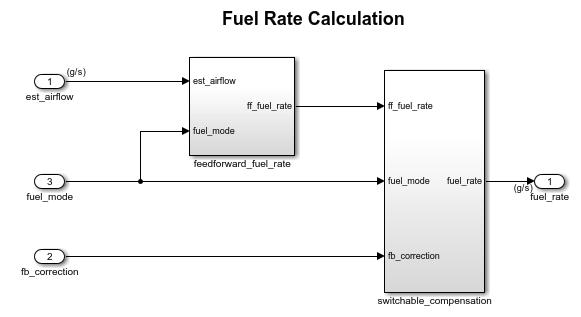
\includegraphics[width=0.7\linewidth]{src/pic/simulink}
    \caption{Simulink schema example.}
    \label{fig:simulink}
\end{figure}

Simulink has plenty of tutorials in many different areas with detailed description and videos on solving it which describes it step-by-step. It is very helpful to have step-by-step solution with detailed description for understanding all important details. Because on this understanding of essentials, is build the future knowledge and depends future success. But there is some weakness in an education process. The issue is, that they don't have methods for validating the correctness of the user's solution and does not encourage the users to try it out by themselves, just copy the sample solution.

\section{Rust} \label{sec:rust}
Rust(Link) is a very popular programming language the prevalence of which is growing every day. It has a consistent tutorial which describes language constructs with gradually increasing complexity. It has the informative and structured index, where users can easily jump from one topic to another almost instantly and then just go back to the place where he was reading before. They use highlighted ares to show some code examples, which facilitate understanding of presented materials. It is possible to copy some parts of the code and even directly execute it in a browser(see figure \ref{fig:rust}).

\begin{figure}[h!]
    \centering
    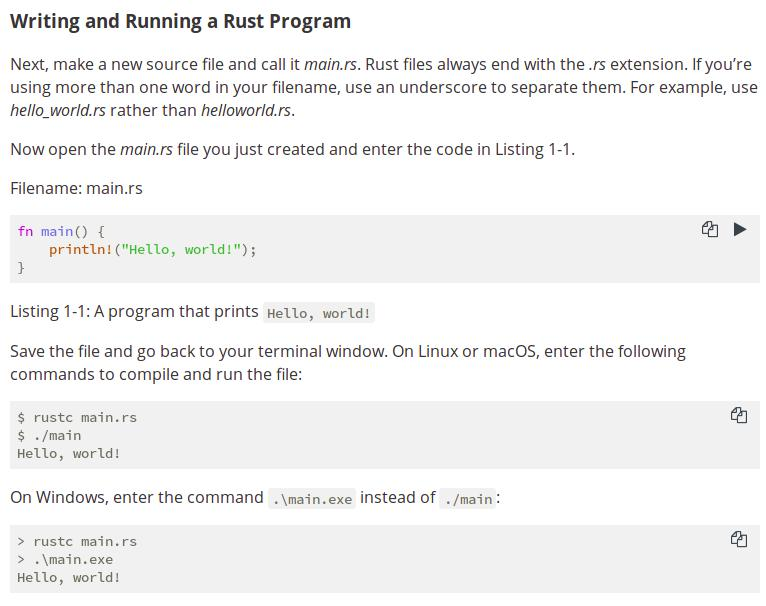
\includegraphics[width=0.7\linewidth]{src/pic/rust}
    \caption{Rust tutorial example.}
    \label{fig:rust}
\end{figure}

To execute the given code, you just have to click on the play button in the upper right corner and in several second the result will be displayed. This is very important and useful feature, because students can directly see what the code does. At the given example it is pretty straightforward, but if you have some computation, not even complex one, it is already not so easy to imagine the output.
Nevertheless, even in this short example, there is some issues related to the compilation process. Namely, the different compilation and execution process for diverse platforms(Windows, Linux, macOS). It means, that we have to install the compiler to use it during the learning process. It would be very convenient to have all these features directly in the web-browser, without installation.

\section{Microsoft Z3 Solver} \label{sec:z3}
Z3 is a state-of-the art theorem prover from Microsoft(link). It provides similar experience compare to Rust tutorial but with some improvements, which simplify the studying process. There is a possibility, not only to execute the given code from the current example directly in the browser, but edit the code, and still see the result almost instantly due to in-browser execution. It helps to see the direct binding between written commands and the real result, that improves understanding of given material.

\begin{figure}[h!]
    \centering
    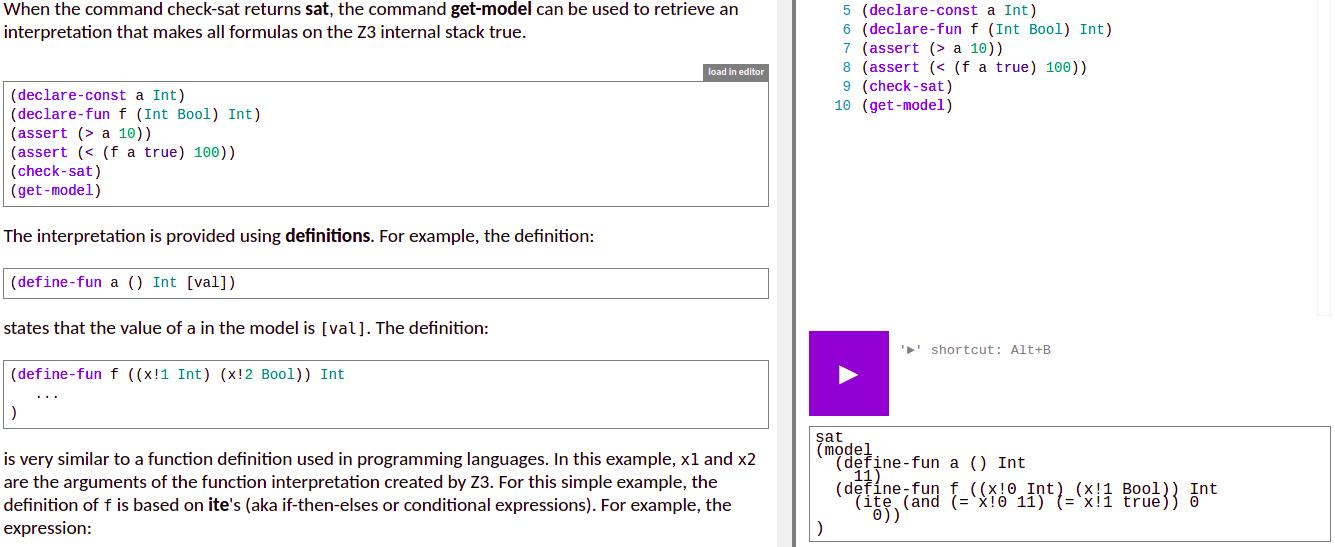
\includegraphics[width=\linewidth]{src/pic/z3}
    \caption{Z3 tutorial example.}
    \label{fig:z3}
\end{figure}

In the figure \ref{fig:z3}, you can see the code given in a tutorial on the left hand side. On the right hand side, there is the code which has been executed and the result appeared below. Then you can adjust the code to check some hypothesis, and instantly see the result. By doing this, students can check their understanding of an explained material.
Another advantage in this tutorial is a in-browser execution. Students do not have to install anything and can directly work in browsers. It means, the operating system(OS) does not have any influence on the execution and compilation process. Any OS can be used, it is necessary to have a web-browser. If this tutorial will be used directly on a lecture, then students just enter the URL in a browser and can instantly try to execute some examples.

\section{Octave Online} \label{sec:octave}
Octave Online(link) is a web-playground fot a high-level language Octave, which is primarily intended for numerical computations. It has a simple and intuitive interface despite the complexity of the internal implementation. It provides directly in a browser fast execution with errors handling. Even if you do complex computations it is not needed to install any software on the PC. Everything works out of the box.

\begin{figure}[h!]
    \centering
    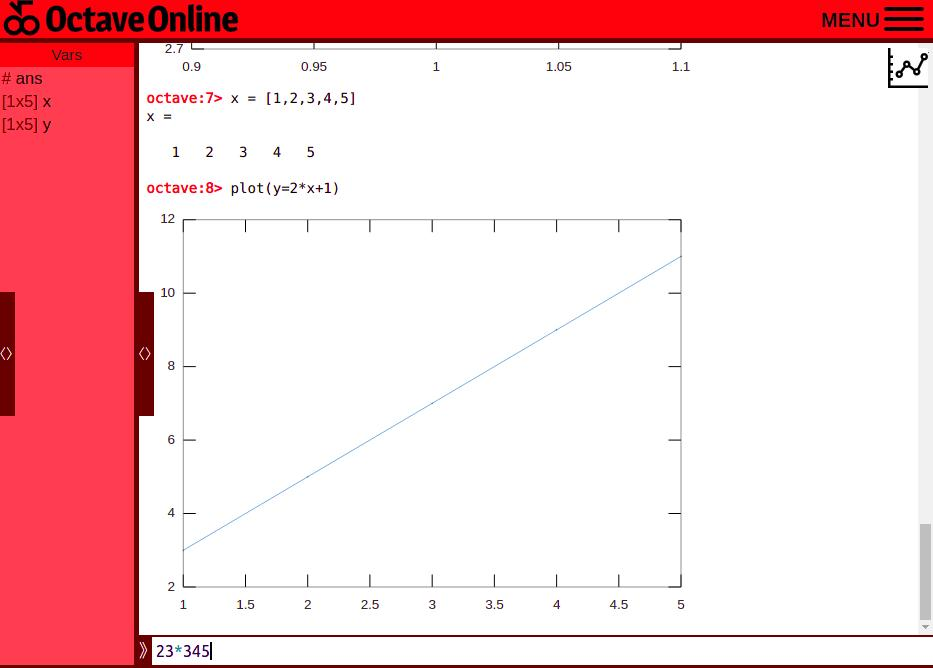
\includegraphics[width=0.7\linewidth]{src/pic/octave}
    \caption{Octave web-playground example.}
    \label{fig:octave}
\end{figure}

This web-playground is oriented on students, who are using the tool directly on the lecture. Do some computations in a browser and run previously created scrips, as a sequence of the commands. To visualize some data, there is a possibility to build some plots for better understanding.

\section{Wolfram Alpha} \label{sec:wolfram}
Wolfram Alpha is a very powerful tool, which works by using expert-level knowledge and algorithms to automatically answer questions, do analysis and generate reports. It has matrix operations and calculations as the EmbeddedMontiArcMath(link) language has, to describe atomic components. It can do even more as solving linear equations, it allows to specify the behavior of controllers, and then, by solving the equations, they synthesize the controller. Furthermore, it has one very interesting and useful feature, which provide the interactive visualization of the given data. The idea behind that is that you can \"feel\" how one or another parameter influence on the final result. It promises a better understanding of the dependencies between the components or elements of the system.

\begin{figure}[h!]
    \centering
    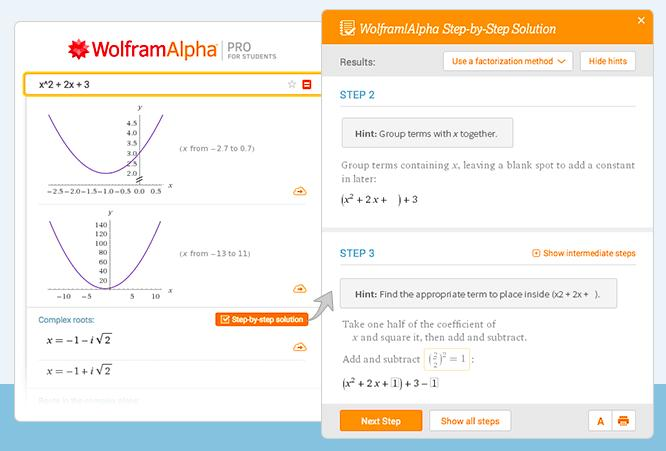
\includegraphics[width=0.7\linewidth]{src/pic/wolfram}
    \caption{Wolfram Alpha example.}
    \label{fig:wolfram}
\end{figure}

It offers the tutorials, which have step-by-step solution with detailed explanation of each step and additional hints for students(see figure \ref{fig:wolfram}). Futhermore, it has high quality visualization, which encourage students to do some experiments and see the changes on the displayed figure.

\section{TypeScript Playground} \label{sec:typescript}
TypeScript is a typed superset of JavaScript. It has a clean and simple playground which shows the difference and benefits of TypeScript over JavaScript. It has preloaded examples which actually show this difference and a user can see distinction in the direct comparison(see figure \ref{fig:typescript}). What, again, gives the better understanding and facilitates further analysis.

\begin{figure}[h!]
    \centering
    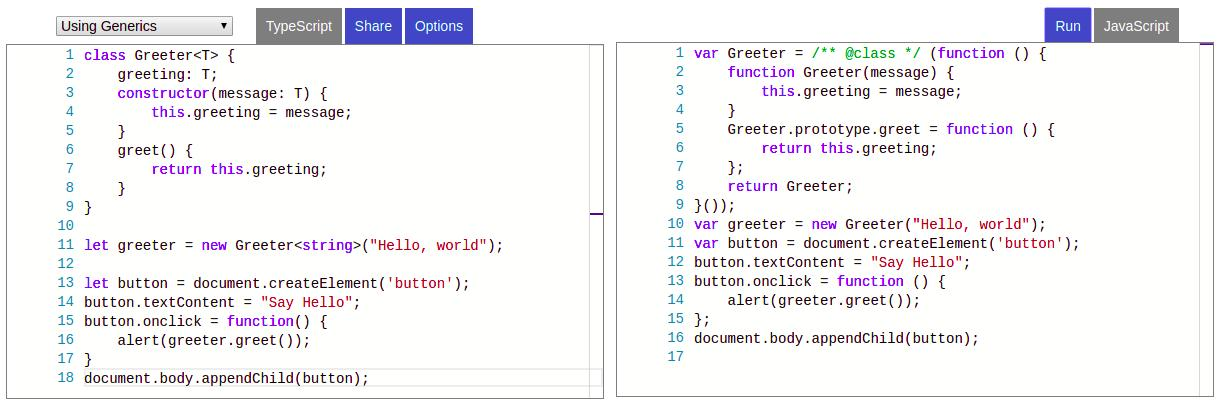
\includegraphics[width=\linewidth]{src/pic/typescript}
    \caption{Typescript playground example.}
    \label{fig:typescript}
\end{figure}

In the picture, it emphasizes the difference in classes architecture. It helps to find architecture advantages of using new language(means Typescript). Moreover, you can run the given example and see the result directly in a browser, but in different tab, which is not really convenient. If you have some complex code, it is really helpful to see the source and the result simultaneously.

\section{Swift Playground} \label{sec:swift}
Swift Playground has been created for teaching the Swift language in a game form. You can create small programs that instantly show the results of the code that you write. From the right side of the screen is shown a 3D world where an action is happen(see figure \ref{fig:swift}). The tutorials are pretty simple but the concept is very interesting. They have automatic verification of an implemented correctness in the 3D environment. To produce many diverse game oriented tutorials, it would be convenient to have simple 3D models importing which can use different models from various 3D editors.

\begin{figure}[h!]
    \centering
    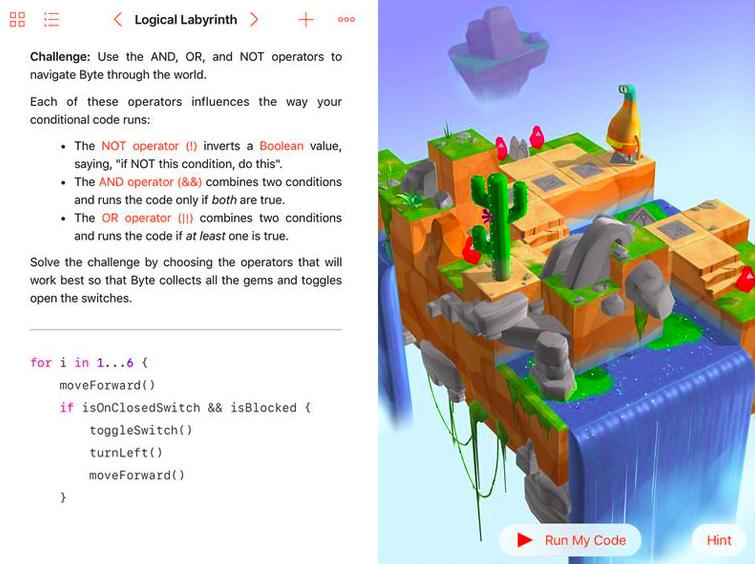
\includegraphics[width=0.6\linewidth]{src/pic/swift}
    \caption{Swift playground example.}
    \label{fig:swift}
\end{figure}

Apple gives into trends and have used the gamification in the tutorials, to attract learners to their product.

\section{Requirements deriving}
Thoroughly analyzed the projects described above, the following list of requirements has been derived: \\\\
(R1) 3D visualization for demonstration purposes \\
(R2) Simple, clean and intuitive interface \\
(R3) Work on any operating system and without installation \\
(R4) Automatic verification of obtained results \\
(R5) Import and use existing 3D models for the simulation \\
(R6) Displaying the object's trajectory \\
(R7) Integrated testing support \\

The table summarizes the comparison between the all considered tutorials. \\
\begin{table}[h!]
    \begin{tabular}{|l|l|l|l|l|l|l|l|l|}
    \hline
    &  Z3 Solver & Octave & Wolfram & TypeScript & Swift & Rust & Simulink & EMAM PG \\ \hline
    R1 & - & + & + & - & + & - & + & + \\ \hline
    R2 & + & + & + & + & + & + & + & + \\ \hline
    R3 & + & + & + & + & - & + & - & + \\ \hline
    R4 & - & - & - & - & + & - & + & + \\ \hline
    R5 & - & - & - & - & - & - & + & + \\ \hline
    R6 & - & - & P & - & P & - & P & + \\ \hline
    R7 & - & - & - & - & - & - & + & + \\ \hline
    \end{tabular}
\end{table}
(+ support, P partially support) \\

Take a closer look at the differences between the tutorials regarding to the derived requirements.\\
(R1) 3D visualization for demonstration purposes: Four considered tutorials have a 3D visualization. The Octave online has a possibility to generate plots and graphics for given data. The Wolfram Alpha has a very powerful tool which can generate 3D models and you can even interact with them and see the changes in a real time. Whereas the Swift Playground has the most advanced 3D world which is like a part of the tutorial and result presentation. The Simulink has an opportunity to build nice 3D models which involved in the simulation process, but the difference is that a user has to build everything himself.\\
(R2) Simple, clean and intuitive interface: This is the only requirement which all tutorial are satisfied. We believe that it is very important to have an understandable and clear interface which does not distract from the educational process. Moreover, the interface should be intuitive so that students can use it directly at the lecture without detailed explanation of its features. \\
(R3) Work on any operating system and without installation: Almost all examined tutorials have web-implementation and work without installation, except the Swift tutorial and Simulink. The Swift tutorial has only iOS implementation. The Simulink does not work on the Web too, only the MathLab, which has partial web-implementation.\\
(R4) Automatic verification of obtained results: Only one among the examined tutorials, the Swift tutorial, has a gaming base verification of a solution correctness. It causes additional interest in the studying process, and can be the motivation to keep solving the tasks, by analogy with computer games. Whereas the Simulink gives you possibility to do it, but it is more like extra feature which can be implemented.\\
(R5) Import and use existing 3D models for the simulation: Only the Simulink has feasibility to import 3D models. It helps to create tutorials quickly and efficiently, by using the previously created models and configurations. An example of reusing a 3D object can be a cone that is used in many exercises. This feature simplifies the process of creating new tutorials and decreases the time which has to be invested into the building process.\\
(R6) Displaying the object's trajectory: Wolfram Alpha, Swift PG and Simulink, we could say, partially support this feature in case that you can see the whole process of movement of the object from the very beginning to the end. But it would be better to improve the concept and add the separate window which permanently displays a traversed route of the object, for better visual perception and visual comparison of results. In our case the object is a car.\\
(R7) Integrated testing support: Only the Simulink has integrated testing options. Due to the specificity of the tutorials, tests play an important role. Writing the streaming test for components, students can be sure that it reacts properly to the incoming data. Tests make the components more reliable and robust. Because of the using the C\&C language, it is great to be sure that each component of a composed model behaves correctly.  
Taking into account all these derived requirements we going to start working on the architecture.\\

\cleardoublepage

\chapter{Preliminaries}
The section introduces technologies that have been used in this thesis. The section \ref{sec:ema} gives an overview of the modelling C\&C language - EmbeddedMontiArc(EMA). The section \ref{sec:tools} presents the whole stack of EmbeddedMontiArc tools that have been used in the toolchain. More detailed description of the tools will be given in the following subsections: the subsection \ref{sec:emam2wasm} EMAM2Wasm describes the generator, which translate code from the EmbeddedMontiArcMath(EMAM) to C++ and then to Web-assembly. The subsection \ref{sec:onlineide} gives an overview of the Online IDE, which is used for writing EMA code in a browser. The subsection \ref{sec:svggen} explains the features of the schema' picture generator.
\section{EmbeddedMontiArc language} \label{sec:ema}
EmbeddedMontiArc language belongs to the MontiCAR language(link) family. It was designed to model architectures of embedded and cyber-physical systems. To show the main advantages of the language, it is easier to start directly with the example \ref{fig:embdmontiarc}.
\begin{figure}[h!]
    \centering
    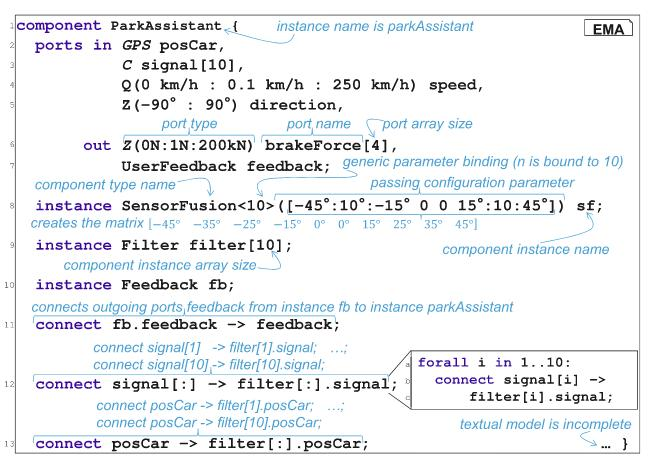
\includegraphics[width=\linewidth]{src/pic/embdmontiarc}
    \caption{Textual EmbeddedMontiArc model of ParkAssistant.}
    \label{fig:embdmontiarc}
\end{figure} \\
In the picture is shown the component with the name - ParkAssistant. This is not the entire component but a main part, which shows the most important features. It has incoming and outgoing ports. All ports must have a type, name and range. The type defines a kind of a signal(e.g., Q,N,Z,B). The range is very important, it helps to control the signal in boundaries, which are defined in advance. Moreover, the range defines not only the boundary values, but the units(e.g., km/h, m/s and so on). Another option, which is available for ports - port size array. It is possibility to define an array of ports, it can increase the readability of the connection schema and simplify the ports connection. When the component is created and ports have been defined, it is possible to instantiate another components inside the component. How you can seen in the lines 8,9 and 10, there are several features available. The first one is to define the generic parameter for a component, to be able create a more general component, which can be used for different types of incoming signal. The next one is to create an array of components, if it is required several similar components for some reason, like the filter component, which does some signal refining. The last one, it is just a normal component instantiation, without any extra parameters. When all required components have been instantiated, it is time to connect the components together. EmbeddedMontiArc offers several convenient options to do that. Firstly you can just connect the specific port of one component to another specific port of another component, like it is shown in the 11th line. Then it is possible to connect an array of ports to another one, to reduce the number of connections between components. Another possibility to connect one port of some component to a specific port of other components, like one-to-many connection. 

\section{EMA Tools} \label{sec:tools}
In this section will be described a full stack of components, which have been used in the toolchain. These components have been developed by other students and in this thesis they will be combined in one chain. The first one is Online IDE, which is used in front end, and another two are EMAM2Wasm generator and SVG generator, which are used in the back end.
\subsection{Online IDE} \label{sec:onlineide}
Online IDE is based on the Cloud9 IDE, that is an online integrated development environment. It supports various languages and was adapted to support the EmbeddedMontiArc and EmbeddedMontiArcMath. It has many features which simplify the development process(see figure \ref{fig:onlineIDE}). The IDE supports the autocompletion for the given languages and syntax highlighting. It increases the speed of the development process and convenience during the code writing. From the left hand side is located the directory tree, which is simplify the navigation inside the project. In this area, you can create new files and folders. Files, which have beed opened, organized in tabs, which can be also used for navigation. From the right hand side, there is shown the list of all ports of the currently selected component. Then the list of the sub-components, which contains the selected component. It shows types of components and their names. When there are many other components in the component, it is easier to see the entire list of components in one screen. Below the sub-components, a group of connectors is shown, which are used to connect currently selected component with others components instantiated inside it. Moreover, the autocompletion is offered to connect to ports of a component, which actually has this component. It means that, the autocompletion tracks all instantiated components with ports. Needless to say, that the IDE supports a text search and search through the ports, sub-components and connectors.
\begin{figure}[h!]
    \centering
    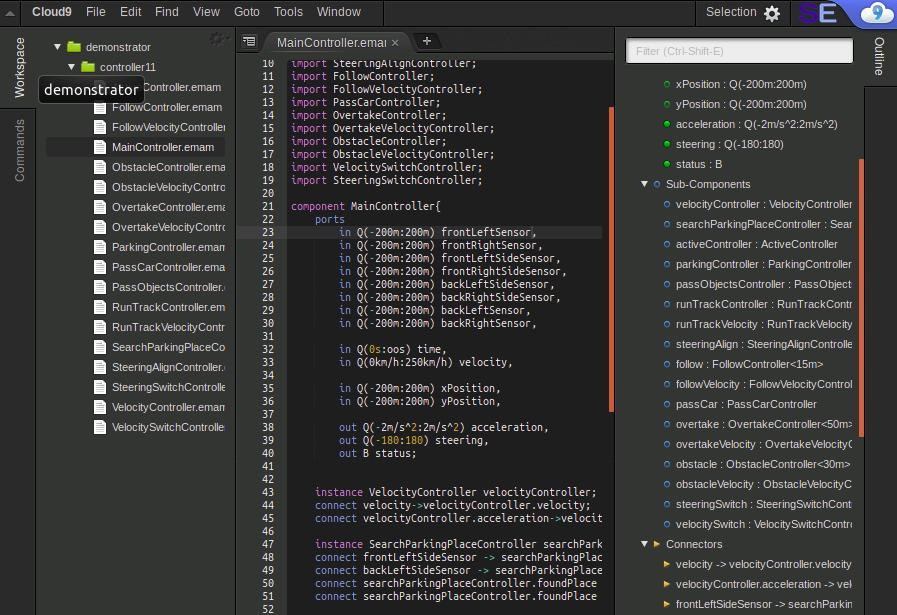
\includegraphics[width=\linewidth]{src/pic/onlineIDE}
    \caption{EMA Online IDE.}
    \label{fig:onlineIDE}
\end{figure} \\
To store porject's files, a virtual file system(VFS)(link) is used. It provides the filesystem API, which is used by developers to manipulate the project's files. It makes available all basic methods for working with files and folders(e.g., mkdir, readFile, copy and so on).
\subsection{EMAM2Wasm} \label{sec:emam2wasm}
This tool generates the web-assembly binary file and JavaScript file from the EMA project. The tool is based on the EMAM2Cpp generator, which firstly produces the c++ equivalent of the EMAM model, afterwards the generated c++ model is used to generate the Web-assembly model, using Emscripten compiler \cite{Emscripten}. The produced files later are used in a browser to execute compiled EMA model for the 3D visualization process. \\
The tool is consisted of the .jar file, which has packed with all dependencies and script files. One of these script files, does the setup procedure and another one executes the main .jar file, with all important parameters. One of the important parameters, which is given in the script file, is a path to Armadillo \cite{Armadillo} library. It is a C++ library for linear algebra \& scientific computing and it is used for matrix computations.
\subsection{SVG generator} \label{sec:svggen}
The main purpose of the SVG generator to create single or multiple layers schema of the given controller. The generated schema helps to visualize the textual model of the EMA controller. The visualization can help to find some errors related to incorrect connection between some components. The SVG generator able to generate multiple layer models, that increases a readability of schemas, because firstly you see more general schema of the model, then you just need to click on some component and an internal schema of the component is appeared.
\begin{figure}[h!]
    \centering
    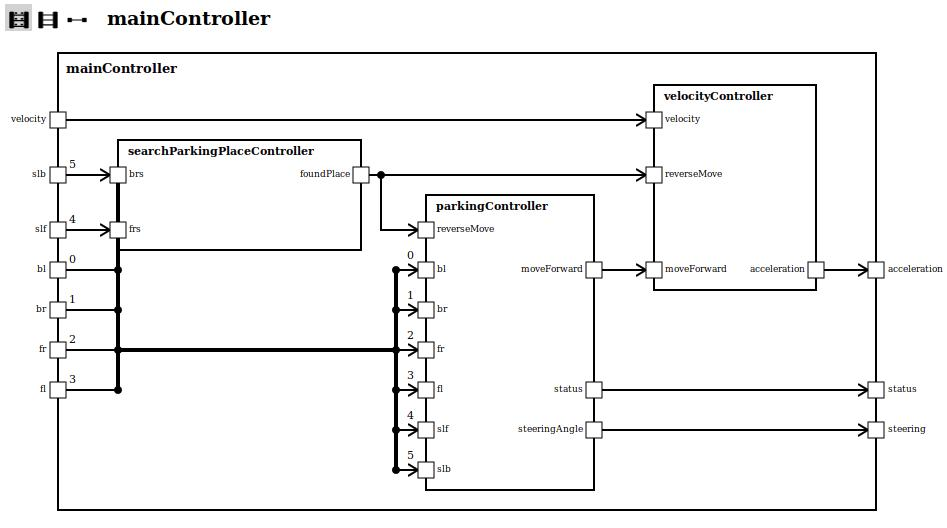
\includegraphics[width=\linewidth]{src/pic/controller03}
    \caption{EMA Parking controller.}
    \label{fig:parkingCtrl}
\end{figure}
In the figure \ref{fig:parkingCtrl} is depicted the parking controller, which has three internal sub-components. Each of these components can have another components inside. The generator calculates the layout in the way to optimize positions of components and decrease the length of the connectors between them. One of the features, is a possibility to simplify the schema by hiding the ports' names and grouping the connections between components.
\chapter{Tutorials}
In this chapter a group of tutorials will be presented. The goal of the tutorials to teach students the basics of the EmbeddedMontiArc language and give a general idea how to build the autopilot's models. The tutorials are given with respect of an increasing the complexity level. Examples are explained step-by-step, to give the best studying experience.
\section{Zero tutorial}
\textbf{Task:} accelerate to the given speed. \newline
Implement the model that continuously accelerates to 10 m/s and then stops.\\ \\
Basic explanation:\\
The car has 8 sensors to measure distances to obstacles. They are located respectively: \\
\begin{figure}[h!]
    \centering
    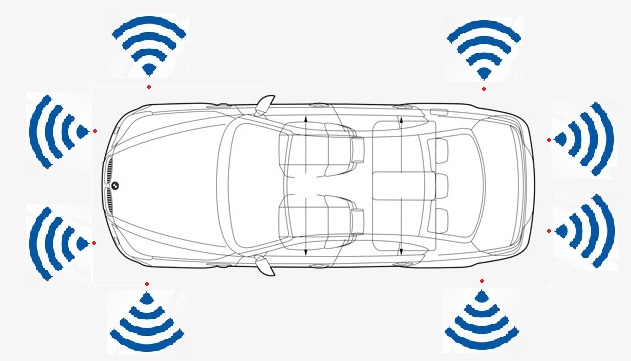
\includegraphics[width=\linewidth]{src/pic/car-with-sensors}
    \caption{Car with sensors.}
    \label{fig:sensors}
\end{figure} \\
To solve this task it's needed to control only an acceleration of the car. Changing the acceleration you may control the behavior of the car. To be able to reach 10 m/s speed, you have to accelerate the car continuously until it reaches the desired speed. Let's start with a MainController which defines the interface to the simulator. We should create a new file which has the same name like component has, with .emam extension.
\bigskip
\begin{lstlisting}
    package controller;

    component MainController{
        ports                                   
            in Q(-200m:200m) frontLeftSensor,
            in Q(-200m:200m) frontRightSensor,
            in Q(-200m:200m) frontLeftSideSensor,
            in Q(-200m:200m) frontRightSideSensor,
            in Q(-200m:200m) backLeftSideSensor,
            in Q(-200m:200m) backRightSideSensor,
            in Q(-200m:200m) backLeftSensor,
            in Q(-200m:200m) backRightSensor,
    
            in Q(0s:oos) time,
            in Q(0m/s:25m/s) velocity,
            in Q(-200m:200m) xPosition,
            in Q(-200m:200m) yPosition,
    
            out Q(-2m/s^2:2m/s^2) acceleration,
            out Q(-180 deg:180 deg) steering,
            out B status;
    ...
\end{lstlisting}
\bigskip
The first eight incoming ports, lines from 5 to 12, receive the data from the sensors which are shown in the picture \ref{fig:sensors}. The next port is a simulation time, which starts from zero second to infinity. The velocity incoming port shows a current velocity of the car. And the next two ports give a position of the car on a track. After the incoming ports the outgoing are following. Outgoing ports control a behaviour of the car using the data which is coming to the incoming ports. The acceleration port controls the velocity, it is like you have two pedals in the car. If you push a brake, you have a negative acceleration. But if you push an accelerator pedal, the car accelerates and velocity has been increased. Then following the steering port, which controls the rotation of the car. And finally the status port, which signals the end of a simulation process. The reason to finish the simulation can be a successful completion of an assignment or violating by the car the track or a map borders. \\
After examination of the example, we should notice:
\begin{itemize}
\item Component has ports incoming and outgoing
\item For each port must be specified a type ( like Q,B) with a valid range.
\item After each port name has to be a comma and the last one must have a semicolon.
\item The possible units are:
    \begin{itemize}
        \item Distance: meters(m), kilometers(km)
        \item Time: seconds(s), minutes(m), hours(h)
        \item Velocity: km/h, m/s
        \item Acceleration: m/s\^2
        \item Rotation: degrees(deg)
    \end{itemize}
\end{itemize}
It was the default interface for the Simulator. It has to be define for all feature controllers. Then you should create your own components which will be connected to the mainController. Let's create a simple component and connect it to the main one. To do that, we have to create a new file .emam with the following content:
\bigskip
\begin{lstlisting}
    package controller;

    component ExampleController {
	    ports
		    in Q(0m/s : 25m/s) velocity,
		    out Q(-2m/s^2:2m/s^2) acceleration,
		    out B status;

	    implementation Math{
		
		    if (velocity <= 10 m/s)
    	        acceleration = 1m/s^2;
    	    else
    	    	status = true;
            end
	    }
    }
\end{lstlisting}
\bigskip
In this component, which is named - ExampleController, are one incoming port and two outgoing ones. Firstly we should reach the speed 10 m/s then stop the simulation. The logic of the controller is implemented inside the Math{} scope. Inside the Math scope you can see if-else-end constructions and the example how to use it. Moreover, it the Math scope can be used different constructions, which you will see later in the next tutorials. The logic in this controller pretty straightforward, it the velocity of the car is less then 10 m/s then accelerate the car with the acceleration 1 m/s. When the given velocity is reached, stop the simulation by setting the status port to true. \\
When we have created the ExampleController we should import it into the MainController and then instantiate it, to have possibility to use it, like a part of the MainController:
\bigskip
\begin{lstlisting}
    package controller;

    import ExampleController;

    component MainController{ 
    ...

    instance ExampleController exampleController;
    ...
\end{lstlisting}
\bigskip
How you can see, we have imported the ExampleController in the line 3. Then later, after specifying the ports of the MainController we have instantiate the controller with the type ExampleController and the name exampleController. Now we should connect this controller to the main controller using specified ports.
\bigskip
\begin{lstlisting}
    ...
    connect velocity->exampleController.velocity;
    connect exampleController.acceleration->acceleration;
    connect exampleController.status->status;
}
\end{lstlisting}
\bigskip
We have connected the incoming port - velocity(mainController) to our instantiated controller and it's corresponding incoming port velocity. Then we connected the outgoing port of velocityController.acceleration to the outgoing port of our MainController. And finally the status port of the ExampleController to status of the MainController.\\
Finally the connections scheme should look like is depicted in the figure \ref{fig:controller}.
\begin{figure}[h!]
    \centering
    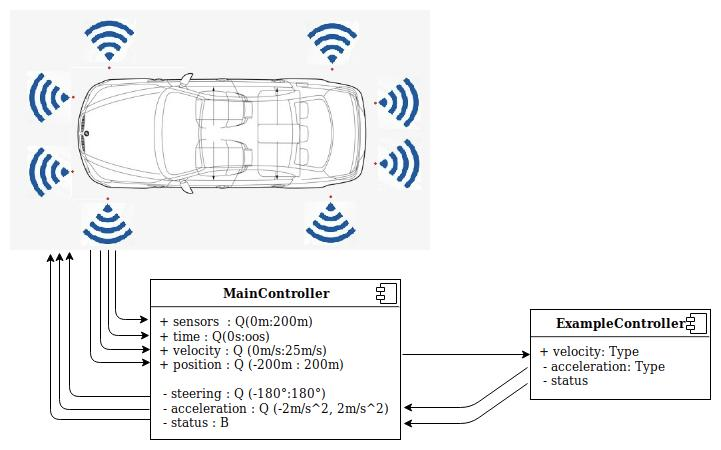
\includegraphics[width=\linewidth]{src/pic/car-with-controller}
    \caption{Car with controller.}
    \label{fig:controller}
\end{figure} \\
Eventually we should send these files to the server to process it and then execute in the simulator, to the how the car behaves using our first controller.
\section{Parallel parking tutorial}
\textbf{Task:} To carry out a parallel parking between two cars. \newline
Implement a model that manages a parking between two cars. The model has to have several modules which are responsible for different actions. One of the examples could be:
\begin{enumerate}
    \item Module which controls the speed of the car, depends on the current action(e.g. parking, searching a parking place).
    \item Module which looking for a gap between cars for the parking.
    \item Module which controls a steering of the car during the parking process.
\end{enumerate}
Each module should be as simple as possible. \newline
To solve this task you should use at least 6 sensors, which measure the distance to objects which are located in front, left side and back of the car. The speed has to be around 0.5-1 m/s. In the picture you can see the main idea how the parking has to be done:
\begin{figure}[h!]
    \centering
    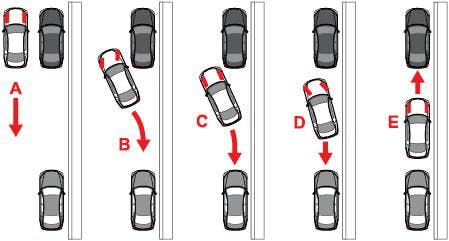
\includegraphics[width=0.8\linewidth]{src/pic/parking_process1}
    \caption{Parking process.}
    \label{fig:parking}
\end{figure}
The parking process can be divided in 4 steps:
\begin{enumerate}
    \item Go straight until a place have been found.
    \item When the place is found, go back and rotate the car.
    \item When the car has reached appropriate point, rotate car in other direction to fit into given gap between the cars.
    \item When the car is close to the car behind, stop and go forward until it reaches certain distance to the front car.
\end{enumerate}
Important to know, this wed-simulator is a simplified version and it does not change the angle of front wheels but an angle of the car entirely. \newline \newline
\textbf{Solution} \newline \newline
To solve that tutorial we have to use the MainController, like we did in the previous tutorial. But we are going to start from an implementation of a controller which will search the place for the car, between two other cars to carry out the parallel parking. The idea is to pass the first car and find the "end" of the second car to start parking process form a right point, like it is shown in the picture \ref{fig:parking}.
\bigskip
\begin{lstlisting}
package controller03;

component SearchParkingPlaceController {
    port
        in Q(-200m:200m) frontLeftSide,
        in Q(-200m:200m) backLeftSide,
        out B foundPlace;

    implementation Math{
        
        static Q passed0 = false;
        static Q passed1 = false;
        static Q passed2 = false;
        static Q passed3 = false;

        if ((backLeftSide - frontLeftSide) > 3m)
            passed0 = true;
        end

        if (((frontLeftSide - backLeftSide) > 3m) && passed0)
            passed1 = true;
        end
        
        if (((backLeftSide - frontLeftSide) > 3m) && passed1)
            passed2 = true;
        end
        
        if (((frontLeftSide - backLeftSide) > 3m) && passed2)
            passed3 = truetutorials/controllers/controller03/SearchParkingPlaceController.emam;
        end
        
        foundPlace = passed3;
    }
}    
\end{lstlisting}
\bigskip
We are using the side sensors to measure the distances to the cars and the side of the road. Using static variables we can save the states(e.g. the distance has changed from 5m to 1m and then from 1m to 5m, it means we have passed the car). Static variables initialized only once. Now we should create a VelocityController, which controls the speed of the car, during the search parking place process and parking.
\bigskip
\begin{lstlisting}
    package controller03;

    component VelocityController {
        port                                    
            in Q(0km/h : 250km/h) velocity,
            in B reverseMove,
            in B moveForward,
            out Q(-2m/s^2:2m/s^2) acceleration; 
    
        implementation Math{                    
    
            if (velocity > 1 m/s)
                acceleration = 0m/s^2;
            else
                acceleration = 1m/s^2;
            end
            
            if reverseMove
                acceleration = -0.5 m/s^2;
            end
            
            if (velocity < -0.5 m/s)
                acceleration = 0m/s^2;
            end
            
            if (reverseMove && moveForward)
                acceleration = 0.5 m/s^2;
            end
            
            if (reverseMove && moveForward && (velocity > 0.5 m/s))
                acceleration = 0m/s^2;
            end
        }
    }
\end{lstlisting}
\bigskip
The velocityController has several different states. The first one is a limit for the velocity during searching parking place (1m/s). The next one is the velocity limit during the reverse move, -0.5 m/s it means, that car moves back. The last one, when the car moves forward during the parking process to move closer to the front car. Next controller will be the most important one, because it manages the parking process.
\bigskip
\begin{lstlisting}
package controller03;
component ParkingController {
    port
        in Q(-200m:200m) frontLeftSensor,
        in Q(-200m:200m) frontRightSensor,
        in Q(-200m:200m) frontLeftSideSensor,
        in Q(-200m:200m) backLeftSideSensor,
        in Q(-200m:200m) backLeftSensor,
        in Q(-200m:200m) backRightSensor,
        in B reverseMove,
        out Q(-35deg:35deg) steering,
        out B moveForward,
        out B status;

    implementation Math{
        
        static B forwardState = false;
        
        if reverseMove
            steering = 1 deg;
        else
            steering = 0 deg;
        end
        
        if (reverseMove && (backLeftSensor < 2m))
            steering = -1 deg;
        end
        
        if (reverseMove && ((backRightSensor == backLeftSensor) ||
            ((backRightSensor < 3m) && (backLeftSensor < 3m))))
                forwardState = true;
        end
        
        if (((frontRightSensor < 3m) || (frontLeftSensor < 3m)) &&
            forwardState)
            status = true;
        else
            status = false; 
        end
        
        if(forwardState &&(frontLeftSideSensor > backLeftSideSensor))
            steering = -0.5 deg;
        end
        
        if(forwardState &&(frontLeftSideSensor < backLeftSideSensor))
            steering = 0.5 deg;
        end
        
        moveForward = forwardState;
    }
}
\end{lstlisting}
\bigskip
The idea is that the car is going back until it reached a certain point, changing an angle of the car. When the car is going back and a distance, from the back left sensor to the road border, is less then 2m, start rotate the car in opposite direction until it is in parallel with the road. Then stop when the limit of the back distance is reached and get closer to the front car. All these steps are nicely illustrated in the picture \ref{fig:parking}. Finally we should connect all these controllers to the interface in the MainController.
\bigskip
\begin{lstlisting}
    package controller03;

    import VelocityController;
    import SearchParkingPlaceController;
    import ParkingController;
    
    component MainController{
        ports 
            in Q(-200m:200m) frontLeftSensor,
            in Q(-200m:200m) frontRightSensor,
            in Q(-200m:200m) frontLeftSideSensor,
            in Q(-200m:200m) frontRightSideSensor,
            in Q(-200m:200m) backLeftSideSensor,
            in Q(-200m:200m) backRightSideSensor,
            in Q(-200m:200m) backLeftSensor,
            in Q(-200m:200m) backRightSensor,
    
            in Q(0s:oos) time,
            in Q(0km/h:250km/h) velocity,
    
            in Q(-200m:200m) xPosition,
            in Q(-200m:200m) yPosition,
    
            out Q(-2m/s^2:2m/s^2) acceleration,
            out Q(-180deg:180deg) steering,
            out B status;
    
        instance VelocityController velocityController;
        connect velocity->velocityController.velocity;
        connect velocityController.acceleration->acceleration;
    
        instance SearchParkingPlaceController searchParkingPlace;
        connect *->searchParkingPlace.*;
        
        instance ParkingController parkingController;
        connect *->parkingController.*;
        connect searchParkingPlace.foundPlace-> [
            velocityController.reverseMove,
            parkingController.reverseMove];
        connect parkingController.*->*;
        connect parkingController.*->velocityController.*;
    }
\end{lstlisting}
\bigskip
All Controllers have been instantiated and then connected to the corresponding ports. The star on the line 33 and later means that the ports, which have similar name are connected to each other. The entire connection scheme is depicted in the figure \ref{fig:parking-scheme}.
\begin{figure}[h!]
    \centering
    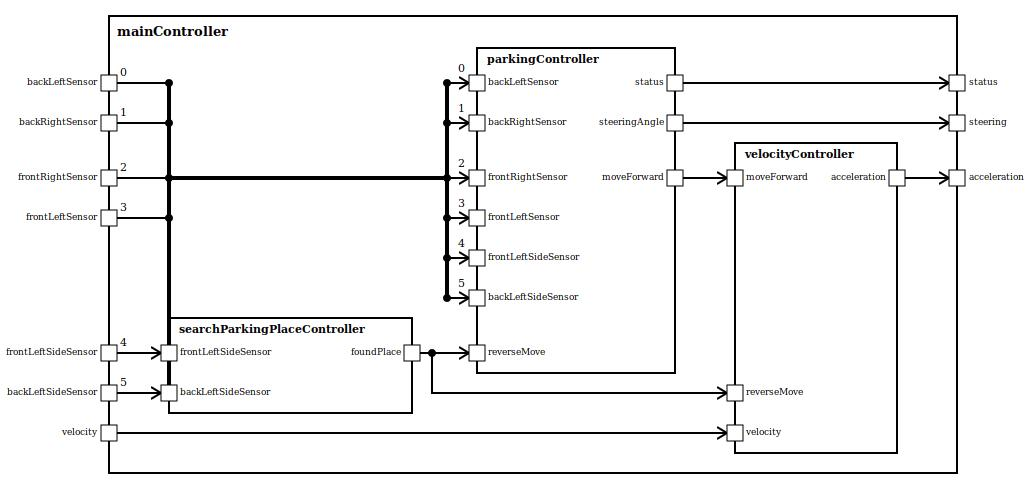
\includegraphics[width=\linewidth]{src/pic/parking-scheme}
    \caption{Parking controller scheme.}
    \label{fig:parking-scheme}
\end{figure}
\section{Maneuverability test tutorial}
\textbf{Task:} Implement a model that manages a driving between cones, which emulates the maneuverability test. The model has to have several modules which are responsible for different actions. One of the examples could be:
\begin{enumerate}
    \item Module controls the speed of the car.
    \item Module is responsible for a steering angle of the car, depends on current position.
\end{enumerate}
Each module should be as simple as possible.
To solve this tutorial you may use from 4 to 6 sensors, which measure the distance to objects which are located in front/side of the car. The speed has to be around 1-2 m/s. In the picture \ref{fig:maneuverability} you can see the main idea how the driving has to be done:
\begin{figure}[h!]
    \centering
    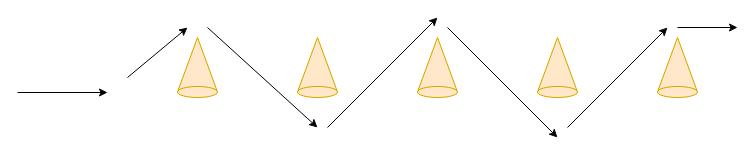
\includegraphics[width=\linewidth]{src/pic/drive_cones}
    \caption{Maneuverability test.}
    \label{fig:maneuverability}
\end{figure} 
The parking process can be divided in several steps:
\begin{enumerate}
    \item Go straight until a cone is closer then 10m then start to rotate the car to round the cone.
    \item When a front part of the car is passed the cone, start to rotate in opposite direction.
    \item When the car is rotated enough to pass the next cone, stop rotation and continue the movement straight.
    \item Repeat the second step until the car passed all cones.
\end{enumerate}
\textbf{Hint:} In this task will be helpful to use the static variables like a counters. \newline \newline
\textbf{Solution} \newline \newline
To solve the given task we should use the MainController, which provides an interface for a communication with the car. Nevertheless, let us start from the Velocity controller, which controls the velocity of the car.
\bigskip
\begin{lstlisting}
package controller04;

component VelocityController {
    ports
        in Q(0km/h : 250km/h) velocity,
        out Q(-2m/s^2:2m/s^2) acceleration; 

    implementation Math{                    

        if (velocity > 1 m/s)
            acceleration = 0m/s^2;
        else
            acceleration = 1m/s^2;
        end
    }
}
\end{lstlisting}
\bigskip
The controller set a limit of the car's velocity on 1 m/s during a process of passing the field of cones. The velocity is controlled by an acceleration. The next controller, which will be implemented, controls a steering of the car to maneuver between cones.
\bigskip
\begin{lstlisting}
    package controller04;

    component ConeRunner {
        port
            in Q(-200m:200m) frontLeftSensor,
            in Q(-200m:200m) frontRightSensor,
            in Q(-200m:200m) frontLeftSideSensor,
            in Q(-200m:200m) frontRightSideSensor,
            in Q(-200m:200m) backLeftSideSensor,
            in Q(-200m:200m) backRightSideSensor,
            in Q(-200m:200m) xPosition,
            out Q(-180deg:180deg) steering,
            out B status;
    
        implementation Math{
            
            static B passRight = false;
            static B passLeft = false;
            static Q(0deg:180deg) count = 0;
            status = false;
    
            if ((frontRightSensor < 10m) && !passLeft && !passRight)
                steering = -1 deg;
            else
                steering = 0 deg;
            end
            
            if (frontRightSideSensor < 1m)
                passRight = true;
                passLeft = false;
                count = 0 deg;
            end
            
            if passRight && (count < 55 deg)
                steering = 1 deg;
                count +=1 deg;
            end
            
            if passRight && (frontLeftSideSensor < 1m)
                passLeft = true;
                passRight = false;
                count = 0 deg;
            end
            
            if passLeft && (count < 55 deg)
                steering = -1 deg;
                count +=1;
            end
            
            if (xPosition > 30m)
                status = true;
            end
        }
    }
\end{lstlisting}
\bigskip
The lines 22-26 are in charge of passing the first cone, because it is located at the center, and the car should behave a bit differently. The car starts rotation to the left slowly, when it has 10 meters to the cone. When it reaches the first cone, it changes the rotation to opposite direction. Then, when it has passed the cone from the right side, it start a rotation to the right using the counter, which is counting the rotation angle to be able to pass a next cone from the left side. There is could be another way of solving this tutorial, without using the counter. The approximate trajectory of the car, you can see in the picture \ref{fig:maneuverability}. The car's rotation varies depending on which side a cone has been passed. After passing the field of cones, the simulation process has been stopped, by using the current position of the car. It happens in the last condition check, line 50. When the controllers, which deliver the main functionality have been developed, we should connect them to the car's interface, which is given in the MainController.
\bigskip
\begin{lstlisting}
    package controller04;

    import VelocityController;
    import ConeRunner;
    
    component MainController{
        ports 
            in Q(-200m:200m) frontLeftSensor,
            in Q(-200m:200m) frontRightSensor,
            in Q(-200m:200m) frontLeftSideSensor,
            in Q(-200m:200m) frontRightSideSensor,
            in Q(-200m:200m) backLeftSideSensor,
            in Q(-200m:200m) backRightSideSensor,
            in Q(-200m:200m) backLeftSensor,
            in Q(-200m:200m) backRightSensor,
    
            in Q(0s:oos) time,
            in Q(0km/h:250km/h) velocity,
            in Q(-200m:200m) xPosition,
            in Q(-200m:200m) yPosition,
            
            out Q(-2m/s^2:2m/s^2) acceleration,
            out Q(-180deg:180deg) steering,
            out B status;
    
        instance VelocityController velocityController;
        connect velocity->velocityController.velocity;
        connect velocityController.acceleration->acceleration;
    
        instance ConeRunner coneRunner;
        connect * -> coneRunner.*;
        connect coneRunner.*->*; 
    }
\end{lstlisting}
\bigskip
In the MainController, firstly we import the implemented controllers then instantiate them and connect. Using the star(*) notation, which is one of the convenient and important feature of the EMA, we can connect all ports with equal names between components. It is simplifies the text model of the controller. If we need to connect only one port, it is better to specify it directly, to facilitate connection's understanding. The entire connection scheme is depicted in the figure \ref{fig:maneuverability-scheme}.
\begin{figure}[ht]
    \centering
    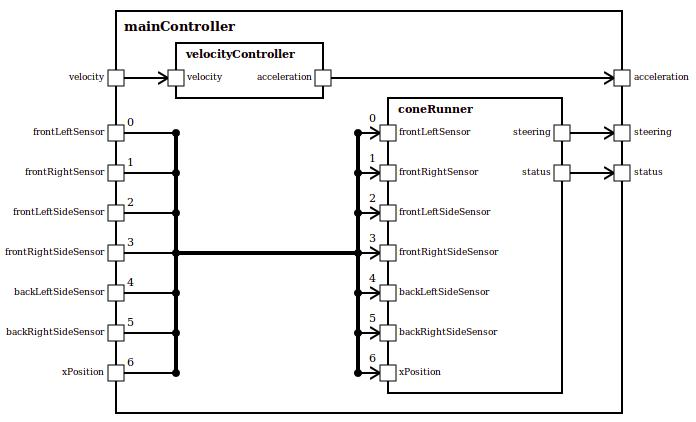
\includegraphics[width=0.8\linewidth]{src/pic/controller04}
    \caption{Maneuverability controller scheme.}
    \label{fig:maneuverability-scheme}
\end{figure}
From the left hand side of the connection scheme, you can see only the ports in the interface, which is indeed connected to other controllers.
\section{Complete track tutorial}
\textbf{Task:} Run through the entire track. \newline \newline
In this tutorial we are going to use previously created controllers to run the track with different obstacles and actions.
\begin{figure}[ht]
    \centering
    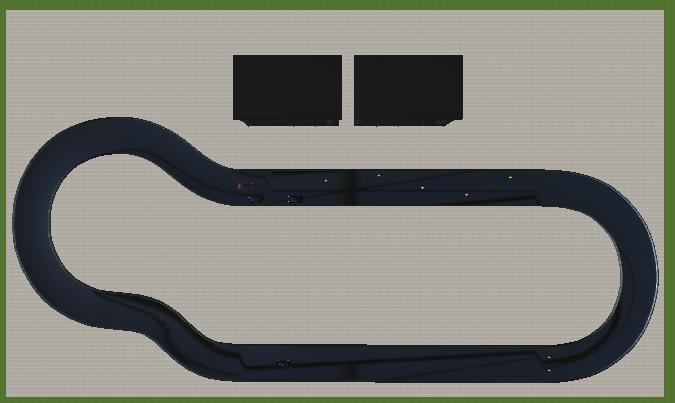
\includegraphics[width=\linewidth]{src/pic/track_tutorial11}
    \caption{Tutorial 11 track.}
    \label{fig:tutorial11-track}
\end{figure}
In the figure \ref{fig:tutorial11-track} the entire track is depicted. We can divide the track into several zones, where different actions are going to happen:
\begin{enumerate}
    \item First one will be the curved area where we have to drive, using our previously created controller for running the whole track with optimal trajectory.
    \item Then on the straight part of the track, a car waiting to start movement, give the possibility firstly to use the follow controller and then the overtaking one.
    \item After overtaking at the end of the strait part of the track, the obstacle form the cones is waiting for the car. The car should brake before the obstacle and then continue the movement when the obstacle is gone.
    \item At the curve part of the track we have to use again, the controller which we used in the first part, just drive through the track.
    \item Next task, will be running across the field of cones.
    \item The last one is the parallel parking. We should use the controller which measure the gap between the cars.
\end{enumerate}
All these controllers were created before in the first ten tutorials and we have to combine all them in one controller which can manage all these actions. Previously we have done some tutorials which use several controllers simultaneously. The main idea that we have an actions controller, which manages actions. This tutorial has to be done in the similar way. \newline \newline
The solution won't be given with the exception of the resulting controller. The controller combines all previously created controllers and will be given in appendix, due to large size of the text model.
\chapter{Toolchain}
In this chapter, will be given a description of the entire toolchain, which is used in the thesis. This toolchain provides the functionality which is required by derived earlier requirements. In the following sections are given the detailed explanation of an architecture and an internal implementation of components from which the toolchain consists.
\section{Architecture}
A software architecture refers to the high-level structures of a software system. The selection of a suitable architecture is very important at the initial design stage. At the very begging, the idea was to create a serverless application which will be hosted on the GitHub pages. And there was a solution for that, at least it looked like the solution. There is a Clang In Browser (CIB)(link) project so you can compile the generated C++ code to web-assembly and run it directly in a browser. But then some issue,related to the solution, has been revealed. CIB does not support dynamic linking yet. Therefore, you cannot link against the large Armadillo mathematics library, which is used by EmbeddedMontiArc and static compilation would extend the linking process to several minutes. Due to this reason, the decision was made to use a stateless server application: a user sends the C\&C files to the server, server translates it to web assembly and then the client receives compiled .wasm controller which is used in the simulator. The huge advantage is that the server is not involved in the simulation process. It means that it is much easier to handle multiple users and it does not run into critical performance issues, due to multiple requests. The simulation in the browser runs fluently, due to local execution for each user and, in our opinion, it has a massive impact on the user experience. Also, the maintenance of a stateless server is much simpler as the maintenance of stateful one. The disadvantage is that users have to wait for the compilation on the server side and it can take longer due to multiple requests. Nevertheless, the user can observe a fluent driving car during the simulation.\newline 
EmbeddedMontiArc has variety of developed tools as self-containing services based on .jar files. Due to the derived requirement R3, it has to be developed a web-based application. Therefore on the server-side, some services, from EmbeddedMontiArcStudio, can be selected and integrated. But still, one server-side component is missing. The server must handle multiple users at the same time, and the server must do the messaging from the back-end to the front-end. Students should get a response from the server, to receive compiled controller or just fix errors which can appear during the compilation process.\newline
The EmbeddedMontiArcStudio has it own 3D simulator, which has a lot of powerful features. But it has some weaknesses, which do not allow to use it in this case. It can not handle multiple users, requires a powerful computer and has to be installed. It contradicts the requirements. Then the decision was made, to develop a new simulator, which satisfies our requirements. For implementation, TypeScript was picked, which is the better version of JavaScript, because it is typed. The simulator which is working on the front-end gives much smoother and fluent experience for a user. Therefore, a fully autonomous front-end is used for the simulator and a back-end during the preparation phase of the controller for the simulator. For the controller of the simulator was decided to use WebAssembly. Web assembly is a new type of code, that runs in modern web browsers. It is a low-level assembly-like language with a compact binary format that runs with near-native performance and provides languages such as C/C++, so that they can run on the web. It is very well suited to this task due to the fact, that it is used EmbeddedMontiArc generator which converts the code to C++. Especially for this purpose, the EmbeddedMontiArc to WebAssembly converter was developed. The architecture more clearly and fully is shown in the figure \ref{fig:architecture}.
\begin{figure}[h!]
    \centering
    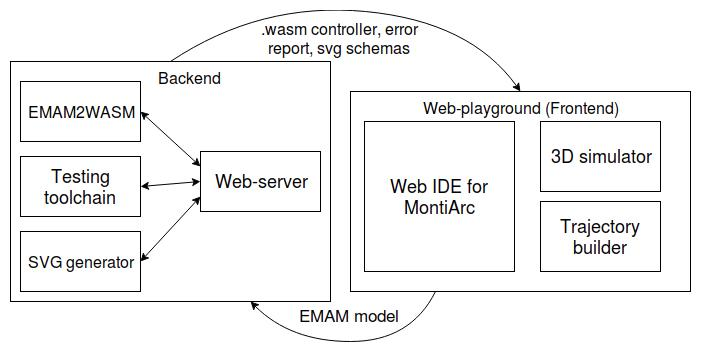
\includegraphics[width=\linewidth]{src/pic/architecture}
    \caption{The toolchain architecture.}
    \label{fig:architecture}
\end{figure} \newline
To clarify the goal of each component which is shown in the picture, it will be considered the seven most important components that are linked together:
\begin{enumerate}
    \item IDE for EmbeddedMontiArc language, it helps to write components easier, reveals the errors and shows incoming and outgoing ports of the components.
    \item Web-server, it receives the requests for compiling the EmbeddedMontiArc models and sends back a finished controller,  packs and extracts models, controls the compilation process, providing an error handling for users. The server has a queue which provides the handling of multiple users simultaneously.
    \item EMAM2Wasm generator, it gets the model from the web-server and compiles it, generating the web-assembly file, which is a "brain" of the simulator.
    \item Testing toolchain, which provides stream testing for incoming models. The toolchain is consist of EMAM2Cpp generator, which generates tests. Then the tests are compiled and executed. The output of the stream testing phase could be used to be shown to the user or be the condition for generating the .wasm file.
    \item SVG generator, it generates a schema of the components and connections for better readability. Users can easier find errors using a schema of components.
    \item Simulator, it receives a compiled model from the server and instantiates it directly in the browser. Then the controller is used to process data from sensors, which located on the car.
    \item Trajectory builder and comparator. It builds in real time a trajectory of the car's movements and does a comparison between a sample trajectory and generated one. The comparator allows having some deviation from the sample trajectory.
\end{enumerate}
In this composition of the components, some of these were reused from the previous successful development. The missing components will be implemented, in the way to accomplish the goal in the most efficient and optimal way.
\section{Front-End}
The Front-End "part" of the toolchain consists of the Online IDE, 3D simulator and trajectory builder. The Online IDE has been already implemented and successful used in production. In the following subsections will be described the main page, which manages a communication with the server, loading of tutorials and files' operations. Then the 3D simulator will be described. It demonstrates the car's behaviour, which is controlled by the compiled model. 
\subsection{Main page}
The main page consists of four iframe tags, which have inside independent web-pages: online IDE, trajectory comparator, 3D web-simulator and description of tutorials. Moreover it ensures the communication between these pages and the Back-End. The functionality which is provided by the main page:
\begin{itemize}
    \item Select and load tutorials. One of the given tutorials can be selected. After that the specified description of the tutorial will be loaded from the server. Due to lack of space on the screen, there is the simulator with the trajectory builder or the tutorial description can be shown, not all together.
    \item Read the data from the Online IDE. It means read files, which were created by the user inside the IDE. All files that were created, are stored in the VFS. If you need to read the data from these files, the special API\cite{FilesystemAPI} has to be used. In this case, an arbitrary number of files and folders can be created. Due to this reason the recursive algorithm has to be implemented for a model reading. Futhermore, JavaScript is an asynchronous programming language and the promises\cite{JSPromise} have to be used, to implement the sequential execution of operations.
    \item Pack files, which have been read, to decrease the size of the blob and amount of transferred files. To pack files directly in the browser, the special library is used. The file reading functionality, which was described above produces an array of the files, which is used by the JSZip library\cite{JSZip} to create a blob.
    \item Send and receive the data to/from the server. When the model has been read and packed, it should be sent to the server for further processing. For this purposes XMLHttpRequest \cite{XMLHttpRequest} is used. It uses POST request to send the blob, which was created by the JSZip library, to the server. The response is sent asynchronously. It means, we can continue to interact with the page during the processing the data by the server. When the data was processed on the server and sent back to the browser, the request object has changed the state to the readyState and it starts to receive the binary data and stores it.
    \item Unpack the incoming data. The browser receives the blob, which is actually just a binary data. Then the blob has to be saved as a .zip archive in the memory. After that, the archive is being extracted. The archive consists of two files. One of them is a .wasm file, which has uint8array encoding. Another one is a .js file, which has string data inside. It is important to differentiate the encoding of these files, due to data consistency inside. During the unpacking process the correctness of received data is checked.
    \item Transfer the compiled model data to the simulator. After the extraction of the received from the server data, the .wasm binary data is validated, by build in WebAssembly validation function. Only after successful validation, the data is being transferred to the 3D web-simulator, where the .wasm controller will be instantiated for further usage.
    \item Load the completed text model of the controller into the IDE. There is possible to load the model, which was implemented as a solution for a tutorial. To load the data to the IDE, the Filesystem API is used, besides, extra functions are required. One of them is cleaning the online IDE environment. It means, delete all files, which were loaded or created earlier. And there is the same issue like we had before with reading. There is no an implemented recursive function, which can do it. And it has to be implemented.
    \item Don't send loaded solution controller to the server if there is no changes in the code. After loading the solution controller, the content of the files can be changed in the IDE. But if the files were not changed, we do not want to spend time waiting the compilation process. Due to this reason, there is pre-compiled controllers, which can be loaded directly to the simulator, to increase usability and convenience of using the product.
\end{itemize}
All described functions have an error handling. If user have some problem with the model, an error message from the server will be received. It is related to all functions which is implemented. It could be an error during packing/extracting process, file reading or .wasm file validation.
\subsection{Tutorial internal structure}
Each tutorial has a textual description, solution and configuration file. The tutorial description has a detailed explanation of the task, which includes some advices and recommendations. The solution gives the step-by-step instructions how to solve the task, and describes why we use particular methods. The configuration files for tutorials have the following data:
\bigskip
\begin{lstlisting}
{
    "car" : 
    {
        "start" : "0:0",
        "end" : "z43"
    },
    "trackObject0" :
    {
        "position" : "100:10",
        "width" : "4",
        "height" : "5",
        "type" : "car"
    },
    "trackObject1" :
    {
        "position" : "z24b",
        "width" : "1",
        "height" : "1",
        "type" : "cone"
    }
}
\end{lstlisting}
\bigskip
The configuration is given in .json format. The first object "car" is the main car, which controlled by a controller. It is possible to define start and end positions. When the car reaches the "end" point, the simulation is stopped. If the simulation should run until a controller terminates the execution, "end" point must not be given. The position of objects can be given as coordinates (x,y) or labels, which are written in the track. The next objects are defined like "trackObject" and have the list of parameters:
\begin{itemize}
    \item Position of the object, which can be given in the same way like "start" point of the car.
    \item Width and height define the size of the object, values given in meters.
    \item Type defines which kind of 3D Objects will be shown in the 3D environment.
\end{itemize}
Usage of configuration files is simplify the creation process for new tutorials and managing of objects on the track. To create a new tutorial, we shouldn't change anything in the simulator, just specify new configuration for the tutorial.
\subsection{3D-web-simulator}
The simulator uses Three.js\cite{ThreeJS}, that is a lightweight cross-browser JavaScript library/API used to create and display animated 3D computer graphics on a Web-browser. This library uses WebGL\cite{WebGL} to increase performance and smoothness of 3D graphics and reduce the intensity of CPU usage, by using the hardware acceleration of the GPU.\newline
To actually be able to display anything with three.js, we need three things: scene, camera and renderer, so that we can render the scene with camera. Then we can add objects to the scene. The most important objects for our tutorials are: track, car and other objects, depends on the task(e.g., cones, cars).\newline
The simulator environment consist of the visual and mathematical model. The visual means the graphical representation, that can be seen in the browser. The mathematical one, it is the model, base on which is built the graphical representation. Then, there is another important part of the chain - controller. The controller was build in advance, before the simulation has been started. In the picture \ref{fig:simulator-scheme} you can see the interaction between the components.
\begin{figure}[h!]
    \centering
    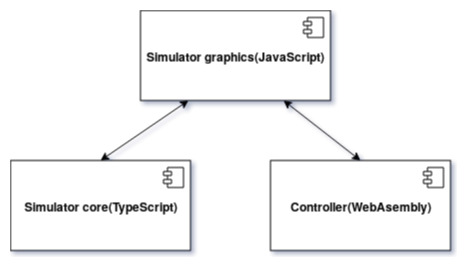
\includegraphics[width=0.7\linewidth]{src/pic/simulator-scheme}
    \caption{The simulator scheme.}
    \label{fig:simulator-scheme}
\end{figure}
\subsubsection{Simulator graphical part}
The graphical part of the simulator is in charge of displaying the simulation process in the 3D environment. The most important part is a main loop. The loop defines how often will be called the move function in the scene, which changes the position of the car in the track. Moreover, inside the loop, the simulator core interacts with the controller. On every cycle, there is the following sequence of actions is taking place:
\begin{figure}[h!]
    \centering
    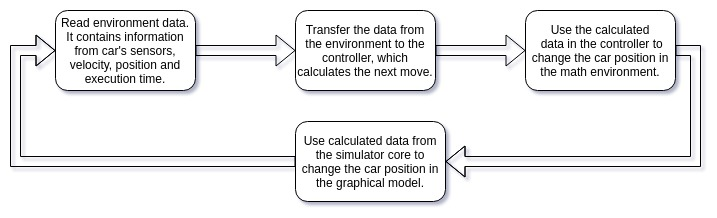
\includegraphics[width=0.7\linewidth]{src/pic/main-loop}
    \caption{The main loop.}
    \label{fig:main-loop}
\end{figure} \newline
There are lots of different functions, which do some service tasks. There is shortly described the most important ones:
\begin{itemize}
    \item Initializing the core simulator and controllers.
    \item Resetting the simulation environment after execution, if it is needed to execute the simulation again. All variables, like execution time or sensor's noise have to be set to initial value.
    \item Reading tutorials' configurations. During loading one of the tutorials, the configuration file is used for instantiation of the track environment. It means, adding the objects to the track and setting up the initial position of the car.
\end{itemize}
The graphical part of the simulator is tightly coupled with the core part. It maps all actions which occurs in the mathematical model to the 3D virtual model, which we can observe. 
\subsubsection{Simulator core part}
Consider the simulator core in more details. The simulator has mathematical model of the track. It means, there is an array of walls, which constantly defined to be equal with the graphical model that was shown during the simulation process. The track has 2 different types of the walls: linear and curved. The linear one is defined by the two points and the curved one has more parameters: start, middle, end points and radius. When the distances to the track's walls have been calculating, in fact, the following occurs:
\begin{itemize}
    \item An intersection of a ray and line is calculated. The initial point of the ray is a sensor position and direction. The line is a wall of the track.
    \item If the intersection was found, then we calculate the distance between the sensor and intersection line. If it was not found, we assume that intersection point exist but with the value Number.MAX\_VALUE.
\end{itemize}
After the calculation of the distances to the track's walls, this data transferred to the controller, which uses it to consider the subsequent behavior of the car. Then the controller passes the result again to the core simulator, which uses this data for further processing. The core simulator has the function - calculate, which uses the data from the controller and executes the next simulation step in the mathematical model. This function controls the main simulation parameters:
\begin{itemize}
    \item Time:
        \begin{equation}
            time = time + samplingTime
        \end{equation} \newline
        where time is simulation time and samplingTime is an increment on each step. 
    \item Velocity:
    \begin{equation}
        velocity = velocity + acceleration * samplingTime
    \end{equation} \newline
        where velocity and acceleration are related to the car.
    \item Rotation:
    \begin{equation}
        rotation = rotation + steering
    \end{equation} \newline
        where rotation and steering angle are related to the car.
    \item Position:
    \begin{equation}
        x = x_0 + velocity * samplingTime * cos(rotation)
    \end{equation}
    \begin{equation}
        y = y_0 + velocity * samplingTime * sin(rotation)
    \end{equation} \newline
    the x0 and y0 are defined the previous position.
\end{itemize}
After the execution of this function, the outgoing data is ready to be used by the graphical part of the simulator and during the next execution step. \newline
\begin{figure}[h!]
    \centering
    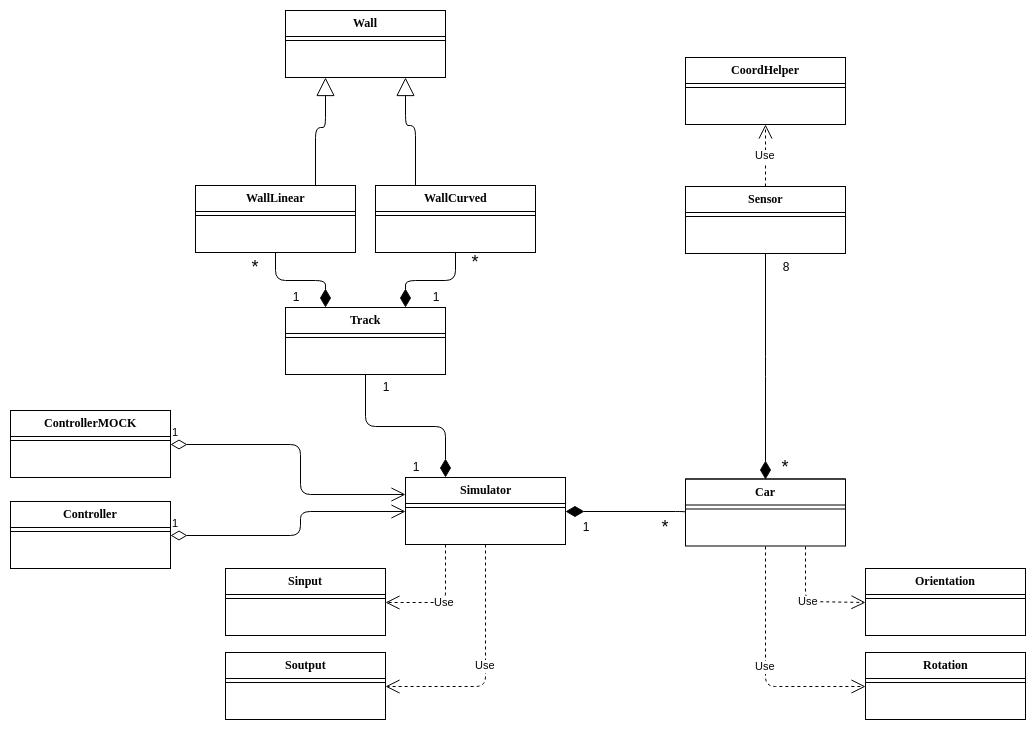
\includegraphics[width=\linewidth]{src/pic/class-diagram}
    \caption{The core simulator class diagram.}
    \label{fig:class-diagram}
\end{figure}
To fully understand how the core simulator works, consider a class diagram \ref{fig:class-diagram}. It depicts classes' dependencies and interaction between them. The main simulator class has a class Track, which has Walls and they can be linear or curved. Moreover, the simulator class has a car, which has eight embedded sensors. The sensors are using the auxiliary class, which helps to calculate the distances. The orientation and rotation classes are used by the car class, to calculate the positions of the sensors when the car changes the angle on the flat. The simulator class uses the structures Sinput and Soutput to fill the input and output data respectively, every execution loop. The simulator works in cooperation with the controller, but for the testing purposes, the MOCK controller has been developed. It helps to test the simulator functionality and body of the MOCK controller can be written in TypeScript.
\subsection{Trajectory builder}
\begin{figure}[h!]
    \centering
    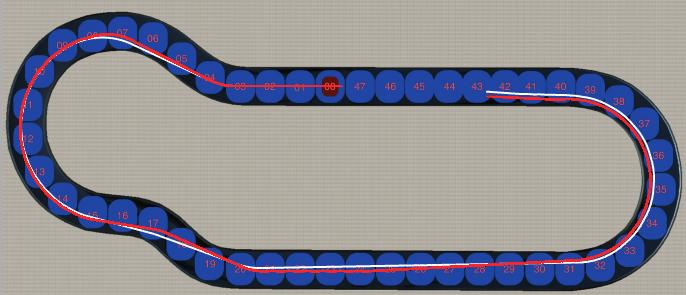
\includegraphics[width=0.8\linewidth]{src/pic/trajectory}
    \caption{Trajectory builder.}
    \label{fig:trajectory}
\end{figure}
Trajectory builder gives a better understanding and a simplicity of analysis the passed way. It is hard to track the whole path of the car and see the controller's errors in real time during the execution. The trajectory helps to solve this problem. In the picture \ref{fig:trajectory} is shown the track with the trajectories. The white one is the sample trajectory while the red one is being drawn in real time, simultaneously with the passing the part of the track by the car. To be able to draw the trajectory a log file is used. It contains all important information about the car in each simulation moment. Information from the log file can be used to analyse the behaviour of the car and reveal problems with the model.
\bigskip
\begin{lstlisting}
logObject.telemetry.push({
  "Status": simulator.output.triggerStatus,
  "Time": simulator.output.ti.value,
  "Position": [simulator.output.xi.value, simulator.output.yi.value],
  "Rotation": simulator.output.degree.value * 180 / Math.PI,
  "Velocity": simulator.output.velocity.value,
  "Sensors": distances
});
\end{lstlisting}
\bigskip
The listing shows the data which is stored in the log. The Time shows the simulation time. Position, rotation and velocity related to the car. The "Sensors" is an array of sensors with measurements in the current simulation point. To build the trajectory, only positioning data is used. The length of the trajectory is calculated by summing up the lengths of all segments between position points. The length between points is calculated using the distance formula \cite{Distance}:
\begin{equation}
    distBetweenPoints += \sqrt{(x_1-x_0)^2 + (y_1-y_0)^2}
\end{equation}
After the summing up all the segments, the \textit{distBetweenPoints} has the entire distance of the track, which is used later to compare the trajectories. To draw the trajectory, all points from the log file are mapped to the picture of the track.
\section{Back-End}
The back-end part of the toolchain is consist of a web-server, EMAM2Wasm generator, testing toolchain and SVG generator. All described component have been implemented and successful used in previous projects. The main goal to connect them all together and implement the web-server, which controls the execution of all services and communicates with the front-end. ?????Additionally, in EMAM language there is a lack of some Context and Conditions checking, which have to be implemented, to obtain better error handling during compilation process.
\subsection{Web-server}
Overwhelming majority of tools related to EMA have been written using Java language and uses the .jar containers. Using .jar container, the applications can be executed on different operating systems, it means they are cross-platform. This is a big advantage, since applications can be run on the server, which does not use Windows, instead some Linux-based system. The web-server is based on the Eclipse Jetty \cite{Jetty}. Eclipse Jetty provides a Web server and javax.servlet container. In our case, we create a server, which bind to the specific port. The servlets' container holds servlets inside, which react on incoming requests from the front-end (see the picture \ref{fig:servlet}). \newline
\begin{figure}[h!]
    \centering
    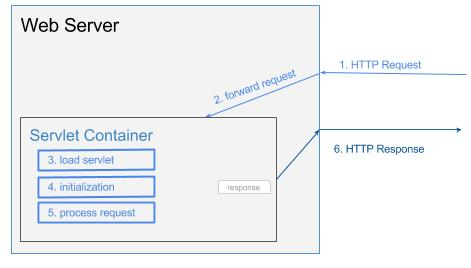
\includegraphics[width=0.6\linewidth]{src/pic/servlet-container-life-cycle}
    \caption{Servlet container.}
    \label{fig:servlet}
\end{figure} \newline
What is really important in our case, that when the request is coming, for each request, a new thread is being created. It means, that we can maintain multiple users, and do not have create manually a multiple user management system. \newline
Then, consider the steps, which occur on the back-end part of the toolchain:
\begin{itemize}
    \item The servler receives the request from the front end. The request contains an archive, which has to be unpacked and the model has to be copied for the further processing. For this purpose, a class has been created, which in charge of unpacking .zip archives and can handle any structure of directories/folders. To decrease a number of I/O operations, the incoming archive is being stored in the RAM.
    \item Then, after the unpacking, the incoming model is being saved to the folder, where models for EMAM2Wasm compiler are located. The compilation process is initiated by executing the particular batch file with parameter, which is a name of the model, that has to be compiled. The butch file initiates the execution of the emam2wasm.jar package. Which has a bunch of parameters e.g., which libraries have to be included, the path to the compiled result and other service parameters, that described in the documentation for EMAM2Wasm \cite{EMAM2Wasm}. The compilation process runs as a separate system process and the web-server receives an output form the process. It means, entire console output is processed by the server and if there is an error, it will be sent to the front-end, to notify the user about the error during the compilation process.
    \item If there is no errors and the model has been successful compiled, it has to be packed to decrease the generated traffic. One of these generated files is a .js file, which actually contains the textual data inside and has high compression rate. Another class, which is in charge of the packing process, packs the data and return the zipStream.
    \item The given zipStream is being written to the response body. The response is marked like a successful performed and is being sent to the front end.
    \item After sending the response, all temporary data on the server will be deleted, to be sure that one day the server will not run out the disc space, due to the large number of compiled models.
\end{itemize}
The web-server, like other EMAM tools is a .jar package and can be installed on different operating systems. Currently, the back end toolchain runs on Windows base OS, but in the future the back end could easily migrate to linux-base environment.
\subsection{CoCo checker}
\chapter{Usage}
Students are going to use the web-playground to understand how to work with C\&C models languages like EmbeddedMontiArc. The main idea of the playground to increase interest in the learning process using a gamification of the tutorials. There are several simple steps in the learning process. The first tutorial is a task which already has a solution but the idea behind that to show the main constructions and principles of the language and the playground. Next tutorials have tasks with increasing complexity and every time there is some hint, which motivates students to use particular constructions. The visualization of the process gives the feeling of the language and understanding of the binding between writing the code and real actions which were caused by the written code. The process of writing tests shows the benefits of test-driven development and understanding the importance of independent testing of the components.
The process of using the web-playground is very simple. Students don't have to install any applications on the computer and it is possible to use it from any platform, whether it is Mac, Windows or Linux. Only one important condition has to be satisfied - to have a "fresh" version of a browser. IDE, tutorial, visualization are located in one window and has a very intuitive interface.
A standard sequence of steps is the following:
1. Open the web-playground in a browser.
2. Read a tutorial
3. Write code with tests
4. Send a model controller to the server, to execute tests and compile the controller.
5. When the simulator displays the ready state, it means that you can run a visualization execution. If the solution contains errors, the student receives an error message with a description.
6. It's possible to restart the simulation process, add some noise to the sensors to emulate more natural measurements, or specify the period of the simulation process. The noise helps students to feel, the influence of the imperfect environment (through a boiling weather or rain) or just a hardware component which has only a certain accuracy. Students learn the difference between plain software engineering (which mostly has no uncertainties) and software systems engineering (which works by interaction with the environment). Also, a controller for embedded systems must be robust, it is another finding that students can learn. A car must continue driving even if it has some inaccuracies in measurements or not critical errors.
7. After the execution, the current trajectory is compared with the sample solution and the student is notified whether he passed the test or not.
The studying process is built on a concept from simple to complex. Doing the tutorials one by one, students get closer to the main goal of the creation of the controller for a self-driving car.